% Options for packages loaded elsewhere
\PassOptionsToPackage{unicode}{hyperref}
\PassOptionsToPackage{hyphens}{url}
\PassOptionsToPackage{dvipsnames,svgnames,x11names}{xcolor}
%
\documentclass[
  openany]{book}
\usepackage{amsmath,amssymb}
\usepackage{iftex}
\ifPDFTeX
  \usepackage[T1]{fontenc}
  \usepackage[utf8]{inputenc}
  \usepackage{textcomp} % provide euro and other symbols
\else % if luatex or xetex
  \usepackage{unicode-math} % this also loads fontspec
  \defaultfontfeatures{Scale=MatchLowercase}
  \defaultfontfeatures[\rmfamily]{Ligatures=TeX,Scale=1}
\fi
\usepackage{lmodern}
\ifPDFTeX\else
  % xetex/luatex font selection
\fi
% Use upquote if available, for straight quotes in verbatim environments
\IfFileExists{upquote.sty}{\usepackage{upquote}}{}
\IfFileExists{microtype.sty}{% use microtype if available
  \usepackage[]{microtype}
  \UseMicrotypeSet[protrusion]{basicmath} % disable protrusion for tt fonts
}{}
\makeatletter
\@ifundefined{KOMAClassName}{% if non-KOMA class
  \IfFileExists{parskip.sty}{%
    \usepackage{parskip}
  }{% else
    \setlength{\parindent}{0pt}
    \setlength{\parskip}{6pt plus 2pt minus 1pt}}
}{% if KOMA class
  \KOMAoptions{parskip=half}}
\makeatother
\usepackage{xcolor}
\usepackage[left=3cm,right=3cm,top=1cm,bottom=2cm]{geometry}
\usepackage{longtable,booktabs,array}
\usepackage{calc} % for calculating minipage widths
% Correct order of tables after \paragraph or \subparagraph
\usepackage{etoolbox}
\makeatletter
\patchcmd\longtable{\par}{\if@noskipsec\mbox{}\fi\par}{}{}
\makeatother
% Allow footnotes in longtable head/foot
\IfFileExists{footnotehyper.sty}{\usepackage{footnotehyper}}{\usepackage{footnote}}
\makesavenoteenv{longtable}
\usepackage{graphicx}
\makeatletter
\def\maxwidth{\ifdim\Gin@nat@width>\linewidth\linewidth\else\Gin@nat@width\fi}
\def\maxheight{\ifdim\Gin@nat@height>\textheight\textheight\else\Gin@nat@height\fi}
\makeatother
% Scale images if necessary, so that they will not overflow the page
% margins by default, and it is still possible to overwrite the defaults
% using explicit options in \includegraphics[width, height, ...]{}
\setkeys{Gin}{width=\maxwidth,height=\maxheight,keepaspectratio}
% Set default figure placement to htbp
\makeatletter
\def\fps@figure{htbp}
\makeatother
\setlength{\emergencystretch}{3em} % prevent overfull lines
\providecommand{\tightlist}{%
  \setlength{\itemsep}{0pt}\setlength{\parskip}{0pt}}
\setcounter{secnumdepth}{5}
\usepackage{booktabs}
\ifLuaTeX
  \usepackage{selnolig}  % disable illegal ligatures
\fi
\usepackage[]{natbib}
\bibliographystyle{plainnat}
\IfFileExists{bookmark.sty}{\usepackage{bookmark}}{\usepackage{hyperref}}
\IfFileExists{xurl.sty}{\usepackage{xurl}}{} % add URL line breaks if available
\urlstyle{same}
\hypersetup{
  pdftitle={BayPass 2.3: tutoriel de génomique d'association adapté au séquençage en pool},
  pdfauthor={Jérôme OLIVARES},
  colorlinks=true,
  linkcolor={Maroon},
  filecolor={Maroon},
  citecolor={Blue},
  urlcolor={blue},
  pdfcreator={LaTeX via pandoc}}

\title{BayPass 2.3: tutoriel de génomique d'association adapté au séquençage en pool}
\author{Jérôme OLIVARES\footnote{INRAE, UR-1115 PSH, 228 route de l'aérodrome, 84914 Avignon, France}}
\date{2023-06-22}

\begin{document}
\maketitle

{
\hypersetup{linkcolor=}
\setcounter{tocdepth}{1}
\tableofcontents
}
\hypertarget{ruxe9sumuxe9}{%
\chapter*{Résumé}\label{ruxe9sumuxe9}}
\addcontentsline{toc}{chapter}{Résumé}

Ce tutoriel détaille d'une part la manière de générer les fichiers d'entrées du logiciel BayPass à partir de données de séquençage en pool, d'autre part le paramétrage optimal du logiciel BayPass et en fin propose une méthode d'exploreration des résultats d'analyses produits. Un pipeline d'analyse mixant des packages sous Rstudio et des lignes de commandes Linux, est décrit afin de guider pas à pas l'utilisateur tout au long du processus depuis les données brutes jusqu'à la liste finale de loci/variants candidats.
Ce tutoriel est à destination des étudiants et des bioinformaticiens débutants.

\hypertarget{mots-clefs}{%
\subsection*{mots clefs}\label{mots-clefs}}
\addcontentsline{toc}{subsection}{mots clefs}

Logiciel BayPass, séquençage en pool, GWAS, études d'associations pangénomiques, Rstudio.

\hypertarget{pruxe9requis}{%
\section*{prérequis}\label{pruxe9requis}}
\addcontentsline{toc}{section}{prérequis}

Les commandes décrites dans cet article ont été regroupées dans un fichier au format « R markdown » (Rmd) « Poolseq\_pipeline.Rmd » librement téléchargeable à l'adresse : \url{https://github.com/Jolivares-INRAE/Download}. Ce tutoriel est conçu pour décrire pas à pas les différentes étapes du fichier Rmd et permettre à l'utilisateur de les exécuter en parallèle.
L'utilisateur devra avoir une connaissance basique du logiciel Rstudio et être capable d'écrire et lancer des scripts sur un cluster de calcul.
Les commandes ont été rédigées sous Rstudio version 1.4.1106 couplé à R 64 bits version 4.0.5. avec toutes les librairies nécessaires à jour (Capture 1) et dans l'environnement bash/SLURM des clusters de calculs de la plateforme GenoToul de bioinformatique (GenoToul Bioinfo ). Dans le cas d'une utilisation dans un autre environnement logiciel, l'utilisateur devra probablement effectuer des adaptations du code.
Bien que l'essentiel des calculs de BayPass seront réalisés sur un cluster de calcul, certains de ses utilitaires seront utilisés en local sous Rstudio, la dernière version du logiciel sera donc téléchargée depuis l'adresse \url{http://www1.montpellier.inra.fr/CBGP/software/baypass/download.html} et décompressée dans un répertoire local par l'utilisateur.
Dans tous les codes qui suivent l'expression « \textasciitilde/path/ » sera à remplacer par les chemins personnels de l'utilisateur.
Le terme de chromosome sera utilisé en références aux appellations de contigs, scaffold, ou chromosomes qui correspondent aux séquences nucléotidiques du génome de référence, plus ou moins mature, qui sera utilisé.

\hypertarget{introduction}{%
\chapter*{Introduction}\label{introduction}}
\addcontentsline{toc}{chapter}{Introduction}

Dans un contexte agronomique actuel de réduction de l'utilisation des pesticides ou de réchauffement climatique, analyser et comprendre les bases génétiques de l'adaptation des organismes aux méthodes de luttes qui leurs sont opposées ou à l'évolution de leur environnement est un enjeu majeur des recherches de ces dernières années.

Les études d'associations pangénomiques (GWAS en anglais pour genome-wide association study) adossées aux techniques de séquençage haut débit (NGS) permettant le séquençage de génome complet, sont un outil de choix pour ce type d'analyse. L'étude au niveau populationnel demandant le séquençage d'un grand nombre d'individus, les couts d'analyses étaient initialement très élevés et ces études étaient souvent réservées aux organismes dit ``modèles'', humain en tête. Néanmoins il a été démontré depuis, que le séquençage en pool d'individus (poolseq) c'est-à-dire en mélangeant de manière équimolaire l'ADN d'un grand nombre d'individus (50 à 100) issus d'une même population permettait non seulement de réduire drastiquement les couts puisqu'on ne réalise qu'un seul séquençage mais aussi que la découverte des points de mutations (SNP) et l'estimation de leur fréquence allélique étaient souvent plus efficaces et précises \citep{futschik_next_2010}. Parmi les logiciels à même d'analyser ces fréquences alléliques on compte Baypass \citep{gautier_genome-wide_2015} qui évalue par une approche baysienne, la différenciation des SNP en liaison avec une covariable environnementale en tenant compte de la structure et de la parenté entre les populations en estimant la covariance (Ω) des fréquences alléliques. Baypass 2.3 a la particularité supplémentaire de pouvoir calculer un contraste des fréquences alléliques entre deux groupes de populations caractérisés par un caractère binaire, sensible ou résistant par exemple.

La documentation disponible de BayPass 2.3 décrit par le menu les algorithmes de fonctionnement et les différents paramètres du logiciel mais reste néanmoins, et assez logiquement, succincte sur les étapes en amont et en aval. A ma connaissance un seul tutoriel est disponible sur le web \citep{nielsen_pool-seq_2020} et décrit de manière plus détaillée la préparation des données brutes et l'analyse en mode « poolseq » de Baypass, mais il nécessite des bases quelque peu avancées de codage sous R et en environnement bash. Si les bio-informaticiens chevronnés ne rencontreront pas de difficultés particulières, il n'en va pas forcément de même pour bon nombre d'agents que les orientations des recherches associées à la baisse des coûts de séquençage ont aiguillé vers les voies de la génomique. Cet article a pour but de détailler les différentes étapes d'une analyse de type GWAS/poolseq avec le logiciel BayPass 2.3 et d'éclairer les points qui sont habituellement peu explicités car considérés comme évident et se veut, au final, le plus proche possible de la citation de Talleyrand : « Si cela va sans le dire, cela ira encore mieux en le disant ».

\hypertarget{pruxe9sentation-du-logiciel-baypass-2.3}{%
\chapter*{Présentation du logiciel BayPass 2.3}\label{pruxe9sentation-du-logiciel-baypass-2.3}}
\addcontentsline{toc}{chapter}{Présentation du logiciel BayPass 2.3}

Le logiciel BayPass est un logiciel de génomique des populations qui vise principalement à l'identification de marqueurs génétiques soumis à la sélection et/ou associés à des covariables spécifiques à la population (variables environnementales, phénotypiques, quantitatives, catégorielles\ldots). Par une approche baysienne il évalue une \textbf{matrice Ω} de covariance des fréquences alléliques des populations résultant de leur histoire démographique. Deux manières d'estimer ces fréquences alléliques sont disponibles soit en se basant sur les génotypes référence/mutant des individus analysés soit, lorsque l'on active le « pool-seq mode », ces fréquences alléliques sont calculées en regard de la profondeur de séquençage (reads count) et pondérées par le nombre d'individus qui ont contribué à cette profondeur. C'est cette seconde approche que nous considérerons dans cet ouvrage.

BayPass propose 3 modèles statistiques d'analyse :

\hypertarget{le-core-model}{%
\subsubsection*{Le Core Model}\label{le-core-model}}
\addcontentsline{toc}{subsubsection}{Le Core Model}

C'est le modèle de base, il permet de calculer la matrice de covariance Ω et d'attribuer une statistique de différenciation XtX à chaque SNP, et ainsi de scanner le génome pour identifier les régions génomiques différenciées entre les populations.Le XtX est une statistique analogue au Fst mais tient compte de la co-évolution des populations grace à la matrice Ω.

\hypertarget{le-standard-model}{%
\subsubsection*{Le Standard Model}\label{le-standard-model}}
\addcontentsline{toc}{subsubsection}{Le Standard Model}

Ce modèle, permet, l'orsque l'on fournit une ou plusieurs covariables (environnementales, phénotypiques\ldots), de calculer un facteur de Bayes, ou Bayes factor en anglais, (BF) pour chaque marqueur génétique représentant la force d'association avec une covariable. C'est un modèle tout en un qui intègre le calcul des XtX et de la matrice Ω, il est adapté au faible nombre de population (\textless{} 15).

\hypertarget{lauxiliairy-model}{%
\subsubsection*{L'Auxiliairy Model}\label{lauxiliairy-model}}
\addcontentsline{toc}{subsubsection}{L'Auxiliairy Model}

Ce modèle a une approche différente dans le calcul de la statistique BF, sans entrer dans le détail il est plus adapté au grand nombre de population (\textgreater{} 15), En contrepartie il nécessite que l'on fournisse une matrice Ω déjà calculée par une analyse Core Model précédente, il recalcule alors les XtX et la statistique BF.

Ces covariables évoquées doivent être distribuées en gradient entre les populations (différence de température, d'altitude\ldots), en complément, dans le cas où la covariable étudiée serait purement binaire (sensible/résistant, gros/petit\ldots), les modèles Standard et Auxiliaire peuvent calculer une statistique C2 qui évalue le contraste de différence des fréquences alléliques de chaque marqueur entre 2 groupes de populations.

\hypertarget{pruxe9sentation-guxe9nuxe9rale-de-lanalyse}{%
\section*{Présentation générale de l'analyse :}\label{pruxe9sentation-guxe9nuxe9rale-de-lanalyse}}
\addcontentsline{toc}{section}{Présentation générale de l'analyse :}

La Figure \ref{fig:Fig1} est une vision simplifiée des différentes étapes nécessaire à l'analyses de données poolseq. Ces étapes se déroulent soit dans l'environnement Linux du cluster de calcul soit sur un ordinateur local sous Rstudio.
La première étape part d'un fichier d'alignement au format « .bam » et consiste à effectuer une recherche de variants (variant calling) pour obtenir un fichier au format « .vcf » de tous les points de mutations ou SNP qui sont autant de marqueurs génétiques à analyser. Ce fichier .vcf sert d'entrée au package « PoolFstat » qui va permettre de générer les fichiers nécessaires au bon fonctionnement de BayPass mais aussi de faire une première analyse des Fst entre populations par exemple. Ces fichiers d'entrées pouvant contenir plusieurs millions de SNP, ils sont découpés en plusieurs dizaines de sous jeux de données afin de réduire les temps de calculs. Une fois que BayPass a analysé tous les sous jeux de données, l'homogénéité des résultats entre eux est analysée sous Rstudio et si tout est bon, les résultats peuvent être regroupés, filtrés et analysés afin de déterminer les marqueurs génétiques et les régions chromosomiques d'intérêts.

\begin{figure}
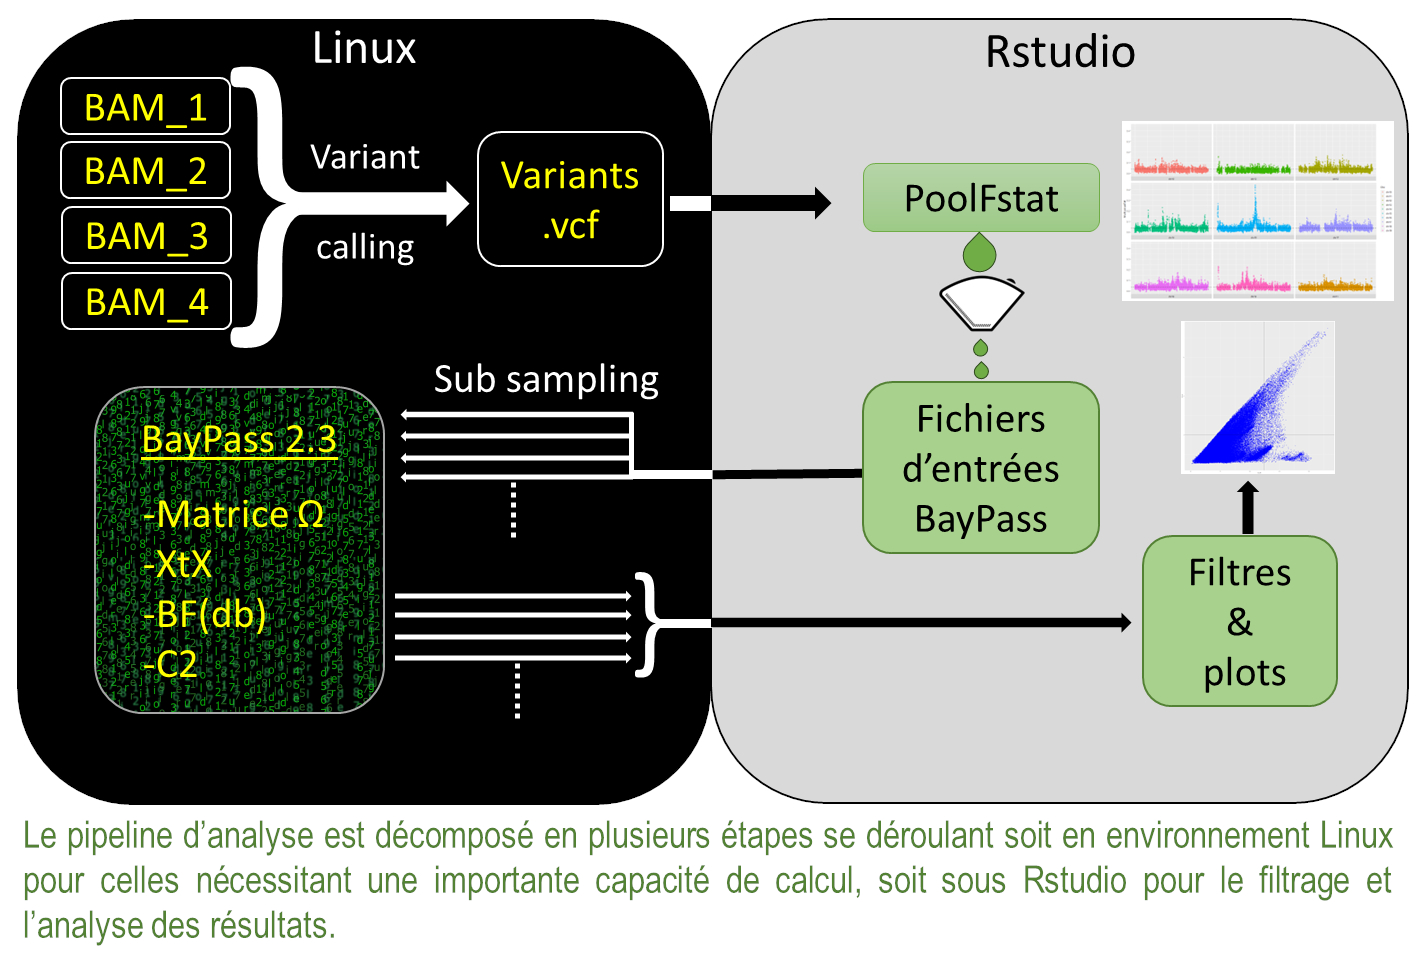
\includegraphics[width=26.07in]{images/Analyse} \caption{Pipeline d'analyses BayPass}\label{fig:Fig1}
\end{figure}

  \bibliography{BayPass.bib}

\end{document}
